\section{Nomenclatura de hidrocarbonetos}
Assim como qualquer outra substância, todo hidrocarboneto precisa de ao menos dois conjuntos de informação: (a) uma fórmula que caracteriza suas propriedades e (b) um nome que define sua unicidade. Uma vez que são conhecidos centenas de milhares de hidrocarbonetos distintos, torna-se obrigatório o uso de alguma sistematização para criação de nomes únicos.

Esta imensa tarefa está centralizada na entidade conhecida como IUPAC (International Union for Pure and Applied Chemistry, ou União Internacional para Química Pura e Aplicada) e está registrada no chamado "BlueBook", documento específico para nomenclatura de substâncias orgânicas.

Devemos alertar o leitor que, uma vez que são conhecidas milhões de substâncias orgânicas, a quantidade de regras e orientações sugeridas pela IUPAC é relativamente grande e abordaremos neste documento, aos poucos, parte dessas regras, pois nossa obra tem escopo bem definido não necessita de todas as regras. Deixamos aqui a curiosidade do leitor na leitura das regras previstas na versão 3 do BlueBook.

São necessários alguns conceitos introdutórios antes de aplicarmos as regras de nomenclatura em Química Orgânica:

\subsection{Cadeia carbônica principal}
Substâncias orgânicas normalmente possuem vários átomos de carbono e em todas elas existe uma \textbf{sequência única de átomos de carbono que é a maior possível}. Esta é a \emph{cadeia principal}. Eventuais átomos ou grupos de átomos que não fazem parte da cadeia principal são chamados de \textbf{radicais}. A figura \ref{fig:23} a seguir ilustra os conceitos necessários para iniciar a compreensão do processo de identificação e numeração da cadeia carbônica principal.

\begin{figure}[H]
	\centering
	\caption{Cadeia carbônica principal e radicais}
	\vspace{0.5cm}
	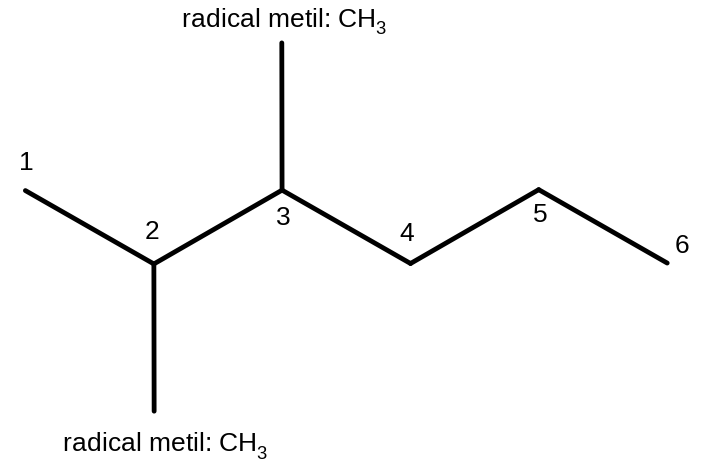
\includegraphics[width=0.75\linewidth]{imagens/23dimetil-hexano.png}
	\label{fig:23}
\end{figure}

Repare que a representação molecular acima é chamada de "bastão" e tem algumas peculiaridades. Nesta representação, as ligações entre átomos de carbono são exibidas como traços (um, dois ou três traços para representar ligações simples, duplas e triplas, respectivamente), em função do caráter covalente dessas ligações, e as ligações entre átomos de carbono e átomos de hidrogênio são \textbf{omitidas} para clareza da representação. As demais ligações precisam ser exibidas.

A cadeia carbônica principal é a maior sequência única de carbonos na molécula, identificada pela sequência numérica de 1 a 6, conforme ilustrado na figura \ref{fig:23} exibida acima. Repare que dois átomos de carbono não fazem parte da cadeia principal e, portanto, são considerados \textbf{radicais}, assim como quaisquer conjuntos de átomos fora da cadeia principal. A nomenclatura de radicais será vista um pouco mais adiante.

\subsection{Radicais}
	
Embora não façam parte da cadeia principal, os radicais fazem parte da molécula e, deste modo, são descritos no nome da molécula. Na figura \ref{fig:23}, temos dois radicais: um deles conectado ao carbono 2 da cadeia principal e outro conectado ao carbono 3. Cada um destes radicais é formado por um átomo de carbono e três átomos de hidrogênio (para completar a tetravalência do carbono), e representados por \textbf{\ce{CH3}}. Este radical chama-se \textbf{metil} e razão deste nome é bem simples: espécies que possuem apenas um átomo de carbono recebem o prefixo \textbf{met}. Além disso, todo radical possui sufixo \textbf{il}.

Muitos dos nomes que você encontrará em livros, apostilas e provas mundo afora são considerados triviais pela IUPAC e os nomes oficiais são, mais uma vez, inequívocos para que você entenda e aplique uma regra sem depender apenas de memória. Veja alguns exemplos:

\textbf{\ce{CH3.}} : esta é a representação sugerida pela IUPAC para o radical metil, uma vez que houve, hipoteticamente, uma quebra homolítica de uma ligação covalente entre carbono e hidrogênio para que se forma o radical citado. Porém, por razões de simplificação didática, o mesmo radical é representado como \ce{CH3-}.

Para deixar ainda mais claro que nomes tradicionais ainda são MUITO utilizados na nomenclatura de substâncias orgânicas, a figura \ref{fig:isopropil} ilustra a estruturas do radical comum em várias substâncias orgânicas e chamado de isopropil (nome tradicional). De acordo com as regras oficiais da IUPAC, o nome oficial do radical é \textbf{propan-2-il}, indicando um conjunto com 3 carbonos (prop), conectados entre si por ligações covalentes simples (an) e o ponto de conexão com um hidrocarboneto pai (cadeia principal ou \emph{parent hydride} na IUPAC) é o carbono central, identificado pelo número 2.
\begin{figure}[H]
	\centering
	\caption{Radical isopropil}
	\vspace{0.5cm}
	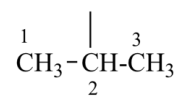
\includegraphics[width=0.25\linewidth]{imagens/isopropil.png}
	\label{fig:isopropil}
\end{figure}